% !TEX program = xelatex
\documentclass[a4paper,10pt]{article}

\makeatletter
\let\@expl@@@mark@update@singlecol@structures@@\relax
\makeatother

\usepackage[a4paper, left=0.95cm, right=0.95cm, top=0.85cm, bottom=0.92cm, footskip=0.52cm]{geometry}
\usepackage{fontspec}
\usepackage{amsmath, amssymb}
\usepackage{longtable, array, colortbl}
\usepackage[table]{xcolor}
\usepackage{fancyhdr}
\usepackage{tikz}
\usetikzlibrary{calc, angles, quotes, arrows.meta, decorations.markings, patterns}

% Cross-platform font discovery (Windows local + Linux repo fonts/)
\makeatletter
\newcommand{\NGSFindFonts}{%
  \IfFileExists{../../../fonts/KhmerOSsiemreap.ttf}{%
    \def\NGSUserPath{../../../fonts/}\def\NGSSysPath{../../../fonts/}%
  }{%
    \IfFileExists{../../../../fonts/KhmerOSsiemreap.ttf}{%
      \def\NGSUserPath{../../../../fonts/}\def\NGSSysPath{../../../../fonts/}%
    }{%
      \IfFileExists{fonts/KhmerOSsiemreap.ttf}{%
        \def\NGSUserPath{fonts/}\def\NGSSysPath{fonts/}%
      }{%
        \def\NGSUserPath{C:/Users/user/AppData/Local/Microsoft/Windows/Fonts/}%
        \def\NGSSysPath{C:/Windows/Fonts/}%
      }%
    }%
  }%
}
\NGSFindFonts
\makeatother

\XeTeXlinebreaklocale "km"
\XeTeXlinebreakskip = 0pt plus 1pt minus 0.1pt

\setmainfont[
  Path = {\NGSUserPath},
  Extension = .ttf,
  UprightFont = KhmerOSsiemreap,
  BoldFont = KhmerOSsiemreap,
  BoldFeatures = {FakeBold=1.8},
  ItalicFont = KhmerOSsiemreap,
  ItalicFeatures = {FakeSlant=0.25}
]{KhmerOSsiemreap}

\newfontfamily\muol[Path={\NGSUserPath}]{KhmerOSmuollight.ttf}
\newfontfamily\Tacteing[Path={\NGSUserPath}]{TACTENG.TTF}
\newfontfamily\enfont[Path={\NGSSysPath}, Scale=1.0]{times.ttf}
\newfontfamily\enbold[Path={\NGSSysPath}, Scale=1.0]{timesbd.ttf}
\newfontfamily\enital[Path={\NGSSysPath}, Scale=1.0]{timesi.ttf}
\newfontfamily\calibrifont[Path={\NGSSysPath}, Scale=0.95]{calibri.ttf}
\newfontfamily\symfont[Path={\NGSSysPath}, Scale=0.95]{cour.ttf}

\DeclareTextFontCommand{\en}{\enfont}
\newcommand{\enbf}[1]{{\enbold #1}}
\newcommand{\enit}[1]{{\enital #1}}
\newcommand{\khmflourish}{{\Tacteing\fontsize{17pt}{17pt}\selectfont 3}}
\newcommand{\wcirc}{{\symfont\char"25CB}}
\newcommand{\chkbox}{\tikz[baseline=0.2ex]\draw[black, line width=0.65pt] (0,0) rectangle (1.45ex,1.45ex);}

\definecolor{headgray}{HTML}{E6E6E6}
\definecolor{stepgray}{HTML}{D4D4D4}
\definecolor{fiveecolor}{HTML}{8B0000}

\pagestyle{fancy}
\fancyhf{}
\renewcommand{\headrulewidth}{0pt}
\renewcommand{\footrulewidth}{0pt}
\fancyfoot[R]{{\calibrifont\fontsize{9.5pt}{11pt}\selectfont\thepage}}

\setlength{\parindent}{0pt}
\setlength{\LTpre}{2pt}
\setlength{\LTpost}{2pt}
\setlength{\tabcolsep}{4.5pt}
\newcolumntype{L}[1]{>{\raggedright\arraybackslash}p{#1}}

\newcommand{\fiveE}[2]{{\color{fiveecolor}\enbf{#1} \enit{(#2)}}}
\newcommand{\timenote}[1]{{\color{fiveecolor}\textit{#1}}}
\newcommand{\stepheader}[1]{%
  \rowcolor{stepgray}%
  \multicolumn{3}{|c|}{\rule[-4pt]{0pt}{15pt}{\muol\fontsize{10pt}{14pt}\selectfont #1}} \\*%
  \hline
}
\newcommand{\cfig}[1]{\begin{center}\vspace{-2pt}#1\vspace{-3pt}\end{center}}

\newcommand{\tri}[1]{\triangle #1}
\newcommand{\unit}[1]{\,\text{\en{#1}}}
\newcommand{\cnum}[1]{\tikz[baseline=-0.58ex]\node[circle, fill=black, text=white, inner sep=0.85pt, minimum size=1.95ex, font=\enbold\scriptsize]{#1};}

% សញ្ញាកែង និងសញ្ញាស្រប ស-ខ្មៅ ច្បាស់ ១០០% (កំណត់ខ្នាត cm ច្បាស់លាស់)
\newcommand{\rightbox}[4][0.20cm]{%
  \coordinate (rbA) at ($(#3)!#1!(#2)$);
  \coordinate (rbB) at ($(#3)!#1!(#4)$);
  \coordinate (rbC) at ($(rbA)+(#3)!#1!(#4)-(#3)$);
  \draw[black, line width=0.65pt] (rbA) -- (rbC) -- (rbB);
}

\tikzset{
  par1/.style={postaction={decorate, decoration={markings,
    mark=at position 0.52 with {\draw[black, line width=0.8pt](-0.06,-0.08)--(0.05,0)--( -0.06,0.08);}}}}
}

% ============================================================================
% ម៉ាក្រូរូបភាព TikZ ស-ខ្មៅ សមាមាត្រច្បាស់ (3.8 cm – 7.2 cm, អក្សរខ្មៅ 100%)
% ============================================================================

% ១. រូបបេសកកម្ម E1៖ ប្លង់ដីកសិដ្ឋាន A និង B ទំ.១៩២ (កែខ្នាត cm មក m តាមបរិបទពិត)
\newcommand{\figEngageAREAThree}{%
\begin{tikzpicture}[scale=0.45, every node/.style={font=\footnotesize, text=black}]
  \coordinate (P1) at (0,0);
  \coordinate (P2) at (5.0,0);
  \coordinate (P3) at (10.4,0);
  \coordinate (Q1) at (0,4.6);
  \coordinate (Q2) at (5.0,3.86);
  \coordinate (Q3) at (10.4,3.06);
  \fill[gray!22] (P1)--(P2)--(Q2)--(Q1)--cycle;
  \fill[gray!08] (P2)--(P3)--(Q3)--(Q2)--cycle;
  \draw[black, line width=1.1pt] (P1)--(P3)--(Q3)--(Q1)--cycle;
  \draw[black, line width=1.0pt] (P2)--(Q2);
  \rightbox[0.20cm]{Q1}{P1}{P2}
  \rightbox[0.20cm]{Q2}{P2}{P3}
  \rightbox[0.20cm]{Q3}{P3}{P2}
  \node[left=2pt] at (0,2.3) {$150\unit{m}$};
  \node[left=1pt] at (5.0,1.9) {$126\unit{m}$};
  \node[right=2pt] at (10.4,1.55) {$100\unit{m}$};
  \node[below=2pt] at (2.5,0) {$120\unit{m}$};
  \node[below=2pt] at (7.7,0) {$130\unit{m}$};
  \node at (2.1,2.5) {\textbf{ប្លង់ $A$}};
  \node at (7.8,1.75) {\textbf{ប្លង់ $B$}};
  \node at (5.2,-1.35) {តើប្លង់ដី $A$ ឬប្លង់ដី $B$ មានផ្ទៃក្រឡាធំជាង? (បាតស្របឈរបញ្ឈរ!)};
\end{tikzpicture}}

% ២. រូប E2៖ ករណីប្រៀបធៀបទីតាំងកម្ពស់ទាំង ៣ តាមឧទាហរណ៍ ទំ.១៩១
\newcommand{\figExploreCasesAREAThree}{%
\begin{tikzpicture}[scale=0.39, every node/.style={font=\footnotesize, text=black}]
  % (ក) កម្ពស់ក្នុង EF
  \begin{scope}[shift={(0,0)}]
    \coordinate (D) at (0,0);
    \coordinate (C) at (4.6,0);
    \coordinate (B) at (3.3,2.7);
    \coordinate (A) at (0.7,2.7);
    \coordinate (E) at (1.8,2.7);
    \coordinate (F) at (1.8,0);
    \fill[gray!14] (D)--(C)--(B)--(A)--cycle;
    \draw[black, line width=1.0pt] (D)--(C) (A)--(B) (D)--(A) (C)--(B);
    \draw[black, line width=0.9pt] (E)--(F);
    \rightbox[0.18cm]{A}{E}{F}
    \rightbox[0.18cm]{E}{F}{C}
    \node[above=1pt] at (A) {$A$};
    \node[above=1pt] at (E) {$E$};
    \node[above=1pt] at (B) {$B$};
    \node[below=1pt] at (D) {$D$};
    \node[below=1pt] at (F) {$F$};
    \node[below=1pt] at (C) {$C$};
    \node at (2.3,-1.55) {(ក) កម្ពស់ក្នុង $EF$};
  \end{scope}
  % (ខ) កម្ពស់ជាជ្រុងកែង AD
  \begin{scope}[shift={(6.0,0)}]
    \coordinate (D) at (0,0);
    \coordinate (C) at (3.8,0);
    \coordinate (B) at (1.8,2.7);
    \coordinate (A) at (0,2.7);
    \fill[gray!14] (D)--(C)--(B)--(A)--cycle;
    \draw[black, line width=1.0pt] (D)--(C)--(B)--(A)--cycle;
    \rightbox[0.18cm]{B}{A}{D}
    \rightbox[0.18cm]{A}{D}{C}
    \node[above=1pt] at (A) {$A$};
    \node[above=1pt] at (B) {$B$};
    \node[below=1pt] at (D) {$D$};
    \node[below=1pt] at (C) {$C$};
    \node at (1.9,-1.55) {(ខ) ជ្រុងកែង $AD$};
  \end{scope}
  % (គ) កម្ពស់ក្រៅ CH
  \begin{scope}[shift={(11.3,0)}]
    \coordinate (D) at (0,0);
    \coordinate (C) at (4.4,0);
    \coordinate (B) at (2.4,2.7);
    \coordinate (A) at (0.7,2.7);
    \coordinate (H) at (4.4,2.7);
    \fill[gray!14] (D)--(C)--(B)--(A)--cycle;
    \draw[black, line width=1.0pt] (D)--(C)--(B)--(A)--cycle;
    \draw[black, line width=0.85pt, densely dashed] (B)--(H)--(C);
    \rightbox[0.18cm]{B}{H}{C}
    \node[above=1pt] at (A) {$A$};
    \node[above=1pt] at (B) {$B$};
    \node[above=1pt] at (H) {$H$};
    \node[below=1pt] at (D) {$D$};
    \node[below=1pt] at (C) {$C$};
    \node at (2.2,-1.55) {(គ) កម្ពស់ក្រៅ $CH$};
  \end{scope}
\end{tikzpicture}}

% ៣. រូប E3៖ សម្រាយបញ្ជាក់ផ្លូវការតាមអង្កត់ទ្រូង AC (ទំ.១៩២)
\newcommand{\figExplainProofAREAThree}{%
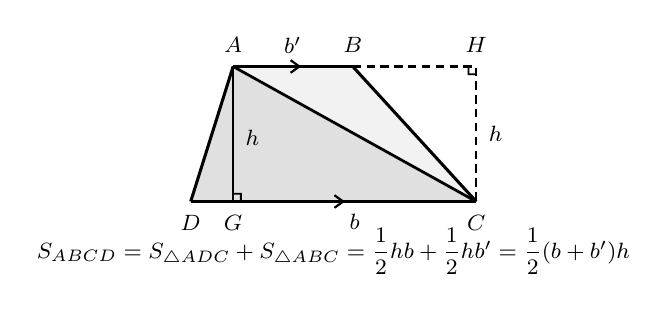
\begin{tikzpicture}[scale=0.49, every node/.style={font=\footnotesize, text=black}]
  \coordinate (D) at (0,0);
  \coordinate (G) at (1.1,0);
  \coordinate (C) at (7.4,0);
  \coordinate (A) at (1.1,3.5);
  \coordinate (B) at (4.2,3.5);
  \coordinate (H) at (7.4,3.5);
  \fill[gray!24] (D)--(C)--(A)--cycle;
  \fill[gray!10] (A)--(B)--(C)--cycle;
  \draw[black, line width=1.1pt, par1] (A)--(B);
  \draw[black, line width=1.1pt, par1] (D)--(C);
  \draw[black, line width=1.1pt] (D)--(A) (B)--(C);
  \draw[black, line width=1.0pt] (A)--(C);
  \draw[black, line width=0.9pt] (A)--(G);
  \draw[black, line width=0.85pt, densely dashed] (B)--(H)--(C);
  \rightbox[0.20cm]{A}{G}{C}
  \rightbox[0.20cm]{B}{H}{C}
  \node[above=1.5pt] at (A) {$A$};
  \node[above=1.5pt] at (B) {$B$};
  \node[above=1.5pt] at (H) {$H$};
  \node[below=1.5pt] at (D) {$D$};
  \node[below=1.5pt] at (G) {$G$};
  \node[below=1.5pt] at (C) {$C$};
  \node[above=1pt] at (2.65,3.5) {$b'$};
  \node[below=1pt] at (4.25,0) {$b$};
  \node[right=1pt] at (1.1,1.65) {$h$};
  \node[right=1pt] at (7.4,1.75) {$h$};
  \node at (3.7,-1.30) {$S_{ABCD} = S_{\tri{ADC}} + S_{\tri{ABC}} = \dfrac{1}{2}hb + \dfrac{1}{2}hb' = \dfrac{1}{2}(b+b')h$};
\end{tikzpicture}}

% ៤. រូប E4៖ លំហាត់គំរូទី ២ ច្រកចូលអគារ (ទំ.១៩៣)
\newcommand{\figModelExAREAThree}{%
\begin{tikzpicture}[scale=0.45, every node/.style={font=\footnotesize, text=black}]
  \coordinate (E) at (0,0);
  \coordinate (D) at (6.0,0);
  \coordinate (C) at (6.0,3.4);
  \coordinate (F) at (0,3.4);
  \coordinate (G) at (1.5,3.4);
  \coordinate (A) at (1.5,5.2);
  \coordinate (B) at (4.5,5.2);
  \fill[gray!12] (E)--(D)--(C)--(F)--cycle;
  \fill[gray!26] (F)--(C)--(B)--(A)--cycle;
  \draw[black, line width=1.05pt] (E)--(D)--(C)--(B)--(A)--(F)--cycle;
  \draw[black, line width=0.85pt, densely dashed] (F)--(C) (A)--(G);
  \rightbox[0.19cm]{A}{G}{C}
  \rightbox[0.19cm]{F}{E}{D}
  \node[above=1pt] at (A) {$A$};
  \node[above=1pt] at (B) {$B$};
  \node[above=1pt] at (3.0,5.2) {$6\unit{m}$};
  \node[left=1.5pt] at (F) {$F$};
  \node[right=1.5pt] at (C) {$C$};
  \node[below=1pt] at (G) {$G$};
  \node[right=1pt] at (1.5,4.25) {$4\unit{m}$};
  \node[left=1.5pt] at (0,1.7) {$8\unit{m}$};
  \node[right=1.5pt] at (6.0,1.7) {$8\unit{m}$};
  \node[below left=1pt] at (E) {$E$};
  \node[below right=1pt] at (D) {$D$};
  \node[below=1.5pt] at (3.0,0) {$12\unit{m}$};
  \node at (3.0,-1.35) {គំរូទី២៖ ច្រកចូលអគារ ($S = 36 + 96 = 132\unit{m}^2$)};
\end{tikzpicture}}

% ៥. រូប E5៖ ប្រតិបត្តិ រូបទី 1 និង រូបទី 2 (ទំ.១៩៣)
\newcommand{\figPracticeEvalAREAThree}{%
\begin{tikzpicture}[scale=0.43, every node/.style={font=\footnotesize, text=black}]
  % រូបទី 1 (កែអក្សរកំពូលស្ទួន B មក D)
  \begin{scope}[shift={(0,0.3)}]
    \coordinate (D) at (0,0);
    \coordinate (C) at (5.2,0);
    \coordinate (B) at (3.7,3.2);
    \coordinate (A) at (0,3.2);
    \fill[gray!22] (D)--(C)--(B)--(A)--cycle;
    \draw[black, line width=1.05pt] (D)--(C)--(B)--(A)--cycle;
    \draw[black, line width=0.8pt] (D)--(B);
    \rightbox[0.19cm]{A}{D}{C}
    \node[above left=1pt] at (A) {$A$};
    \node[above=1.5pt] at (B) {$B$};
    \node[below right=1pt] at (C) {$C$};
    \node[below left=1pt] at (D) {$D$};
    \node[above=1.5pt] at (1.85,3.2) {$10\unit{cm}$};
    \node[left=1.5pt] at (0,1.6) {$6\unit{cm}$};
    \node[below=1.5pt] at (2.6,0) {$x\unit{cm}$};
    \node at (2.15,1.2) {$S=72\unit{cm}^2$};
    \node at (2.6,-1.45) {រូបទី១ ($x = 14\unit{cm}$)};
  \end{scope}
  % រូបទី 2 (ចតុកោណព្នាយភ្ជាប់ការេទ្រេត 30x30)
  \begin{scope}[shift={(7.2,0.3)}]
    \coordinate (P) at (0,0);
    \coordinate (Q) at (5.0,0);
    \coordinate (R) at (3.4,2.6);
    \coordinate (S) at (0.9,2.6);
    \coordinate (H) at (3.4,0);
    % ជ្រុងភ្ជាប់ QR មានប្រវែង sqrt(1.6^2 + 2.6^2) = 3.05 ~ 30 units!
    \coordinate (U) at ($(R)+(2.6,1.6)$);
    \coordinate (T) at ($(Q)+(2.6,1.6)$);
    \fill[gray!18] (P)--(Q)--(R)--(S)--cycle;
    \fill[gray!08] (Q)--(T)--(U)--(R)--cycle;
    \draw[black, line width=1.05pt] (P)--(Q)--(T)--(U)--(R)--(S)--cycle;
    \draw[black, line width=0.85pt, densely dashed] (R)--(H) (R)--(Q);
    \rightbox[0.18cm]{S}{R}{H}
    \rightbox[0.18cm]{R}{H}{P}
    \rightbox[0.18cm]{Q}{R}{U}
    \rightbox[0.18cm]{R}{U}{T}
    \rightbox[0.18cm]{U}{T}{Q}
    \rightbox[0.18cm]{T}{Q}{R}
    \node[above=1.5pt] at (2.15,2.6) {$25$};
    \node[below=1.5pt] at (2.1,0) {$50$};
    \node[left=1.5pt] at (0.42,1.35) {$28$};
    \node[left=1pt] at (3.4,1.3) {$26$};
    \node[below right=1pt] at (6.3,0.75) {$30$};
    \node[above right=1pt] at (6.7,2.4) {$30$};
    \node at (3.8,-1.45) {រូបទី២ ($S=1\,875,\; P=193$)};
  \end{scope}
\end{tikzpicture}}

\begin{document}
\fontsize{10pt}{15.0pt}\selectfont

% ==================== ក្បាលរដ្ឋបាលផ្លូវការ ====================
{\centering
  {\muol\fontsize{11pt}{16pt}\selectfont ព្រះរាជាណាចក្រកម្ពុជា}\\[2pt]
  {\muol\fontsize{11pt}{16pt}\selectfont ជាតិ សាសនា ព្រះមហាក្សត្រ}\\[-2pt]
  \khmflourish\par
}
\vspace{-4pt}
{\muol\fontsize{10pt}{15.2pt}\selectfont
មន្ទីរអប់រំ យុវជន និងកីឡា ខេត្តកំពង់ធំ\\
ការិយាល័យអប់រំ យុវជន និងកីឡា ស្រុកកំពង់ស្វាយ\\
អនុវិទ្យាល័យព្រះក្រសាំង\par}

\vspace{2pt}
{\centering{\muol\fontsize{12pt}{18pt}\selectfont កិច្ចតែងការបង្រៀន}\par}
\vspace{2pt}

{\fontsize{10pt}{15.0pt}\selectfont
\hspace*{3.7cm}%
\begin{tabular}{@{}l l l l@{}}
  - & មុខវិជ្ជា & : & គណិតវិទ្យា ថ្នាក់ទី៨ \\
  - & ចំណងជើងមេរៀន & : & មេរៀនទី១៤ ផ្ទៃក្រឡាពហុកោណ \\
  - & ចំណងជើងរង & : & ៣. ផ្ទៃក្រឡាចតុកោណព្នាយ (ទំព័រ ១៩១--១៩៣) \\
  - & រយៈពេល & : & ១ ម៉ោងសិក្សា (៥០ នាទី) \\
  - & បង្រៀនដោយ & : & ហុក ប៊ុនថែន \\
  - & កាលបរិច្ឆេទ & : & ថ្ងៃអង្គារ ១៣កើត ខែមិគសិរ ព.ស.២៥៧០ (២២ ធ្នូ ២០២៦) \\
\end{tabular}

\vspace{1pt}

% -------------------- I. វត្ថុបំណង --------------------
\textbf{I.} {\muol វត្ថុបំណង}\\[1pt]
\hspace*{0.55cm}%
\begin{tabular}{@{}l l L{14.2cm}@{}}
  \wcirc \hspace{0.25cm} វិជ្ជាសម្បទា & : & សិស្សប្រាប់និយមន័យបាត កម្ពស់កែង (ក្នុង ជ្រុងកែង និងក្រៅរូប) និងទ្រឹស្ដីបទផ្ទៃក្រឡាចតុកោណព្នាយ ($S = \frac{1}{2}(b + b') \times h$) បានត្រឹមត្រូវ ។ \\
  \wcirc \hspace{0.25cm} បំណិនសម្បទា & : & សិស្សស្រាយបញ្ជាក់រូបមន្តតាមការបំបែកអង្កត់ទ្រូងជាត្រីកោណពីរ ($\tri{ADC} + \tri{ABC}$) និងគណនាផ្ទៃក្រឡាចតុកោណព្នាយ រូបសមាស និងរង្វាស់បាតឬកម្ពស់បាត់លើសន្លឹកកិច្ចការបានត្រឹមត្រូវ ។ \\
  \wcirc \hspace{0.25cm} ចរិយាសម្បទា & : & សិស្សមានទម្លាប់ពិនិត្យសញ្ញាបាតស្រប មុំកែង និងវង់ក្រចក $(b+b')$ មុនគណនា ព្រមទាំងសហការផ្ទៀងផ្ទាត់ចម្លើយប្រកបដោយភាពម៉ត់ចត់ ។ \\
\end{tabular}

\vspace{1pt}

% -------------------- II. សម្ភារៈឧបទេស --------------------
\textbf{II.} {\muol សម្ភារៈឧបទេស}\\[1pt]
\hspace*{0.55cm}\parbox[t]{18.2cm}{$\bullet$ \hspace{0.25cm} សម្រាប់គ្រូ៖ សៀវភៅសិក្សាគោលគណិតវិទ្យាថ្នាក់ទី៨ (ទំ.១៩១--១៩៤) ក្ដារខៀន ដីស បន្ទាត់វែង និងសន្លឹកកិច្ចការគំរូ (គ្មានស្លាយ \en{LCD}) ។\\
$\bullet$ \hspace{0.25cm} សម្រាប់សិស្ស៖ សន្លឹកកិច្ចការសិស្ស ស-ខ្មៅ (\en{Worksheet\_AREA3} ២ ទំព័រពេញ) សៀវភៅសិក្សាគោល សៀវភៅសរសេរ បន្ទាត់ក្រិត និងប៊ិច/ខ្មៅដៃ ។}

\vspace{1pt}

% -------------------- III. វិធីសាស្រ្តបង្រៀន --------------------
\textbf{III.} {\muol វិធីសាស្រ្តបង្រៀន}\\[1pt]
\hspace*{0.45cm}%
\begin{tabular}{@{}l l L{14.85cm}@{}}
  $\bullet$ \hspace{0.25cm} គោលវិធី & : & សិស្សមជ្ឈមណ្ឌល (បង្រៀនដោយមិនប្រើស្លាយ \en{LCD} យកសន្លឹកកិច្ចការបំពេញចន្លោះជាគោល) \\
  $\bullet$ \hspace{0.25cm} យុទ្ធវិធីបង្រៀន & : & ស្ថាបនានិយម គំរូ \en{5Es} រួមផ្សំករណីប្រៀបធៀបកម្ពស់ ៣ ទម្រង់ (\en{Contrasting Cases}), ការបំបែកតាមអង្កត់ទ្រូងជាត្រីកោណពីរ (\en{Diagonal Triangulation}) និងការវិនិច្ឆ័យកំហុសគំរូ (\en{Erroneous Examples}) \\
\end{tabular}
}

\vspace{1pt}

% -------------------- IV. ដំណើរការបង្រៀន --------------------
\textbf{IV.} {\muol ដំណើរការបង្រៀន}

\vspace{1pt}

\renewcommand{\arraystretch}{1.15}
\begin{longtable}{|L{5.50cm}|L{7.90cm}|L{4.80cm}|}
\hline
\rowcolor{headgray}
\multicolumn{1}{|c|}{\muol សកម្មភាពគ្រូ} &
\multicolumn{1}{c|}{\muol ខ្លឹមសារមេរៀន} &
\multicolumn{1}{c|}{\muol សកម្មភាពសិស្ស} \\
\hline
\endfirsthead

\hline
\rowcolor{headgray}
\multicolumn{1}{|c|}{\muol សកម្មភាពគ្រូ} &
\multicolumn{1}{c|}{\muol ខ្លឹមសារមេរៀន} &
\multicolumn{1}{c|}{\muol សកម្មភាពសិស្ស} \\
\hline
\endhead

\hline
\endfoot

\hline
\endlastfoot

% ==================== ជំហានទី១ (2min) ====================
\stepheader{ជំហានទី១ ៖ រដ្ឋបាលថ្នាក់ (២ នាទី)}
$\bullet$ ពិនិត្យអវត្តមាន សណ្ដាប់ធ្នាប់ និងអនាម័យថ្នាក់រៀន\par\vspace{1pt}
$\bullet$ ចែកសន្លឹកកិច្ចការ \en{Worksheet\_AREA3} (១ សន្លឹកសងខាង) ដល់សិស្សគ្រប់គ្នា
&
$\bullet$ ពិនិត្យវត្តមាន និងការត្រៀមសម្ភារៈសិក្សា (សន្លឹកកិច្ចការ សៀវភៅសិក្សាគោល និងបន្ទាត់ក្រិត)
&
$\circ$ ប្រធានថ្នាក់រាយការណ៍អវត្តមាន\par\vspace{1pt}
$\circ$ ទទួលសន្លឹកកិច្ចការ និងសរសេរឈ្មោះ \\[3pt]
\hline

% ==================== ជំហានទី២ (9min: ≤3 + 3 + E1 3) ====================
\stepheader{ជំហានទី២ ៖ កែកិច្ចការផ្ទះ រំលឹកមេរៀនចាស់ និងភ្ជាប់មេរៀនថ្មី (៩ នាទី)}
\timenote{(កែកិច្ចការផ្ទះ $\le 3\unit{min}$)}\par\vspace{1pt}
$\bullet$ ហៅសិស្ស ២ នាក់ឡើងសរសេរចម្លើយលំហាត់ទី៧ (រូបទាំងពីរ ទំ.១៩៥) លើក្ដារខៀន
&
\textbf{កំណែកិច្ចការផ្ទះ (ទំ.១៩៥ — លំហាត់ទី៧)៖}\par\vspace{1pt}
១. \textbf{រូបខាងឆ្វេង៖} $S = \frac{1}{2}(4.5)(6.7) = 15.075,\; P = 4(4.0) = 16.0$ ។\par\vspace{1pt}
២. \textbf{រូបខាងស្ដាំ៖} $S = \frac{1}{2}(50)(40) = 1\,000,\; P = 4(32) = 128$ ។
&
$\circ$ សិស្ស ២ នាក់ឡើងបំពេញចម្លើយ និងផ្ទៀងផ្ទាត់ក្នុងសៀវភៅ \\[3pt]

\timenote{(រំលឹកមេរៀនទាក់ទង $3\unit{min}$)} $\bullet$ សំណួរទី១៖ «តើចតុកោណព្នាយមាននិយមន័យដូចម្ដេច?»
&
\textbf{ចំណេះដឹងមូលដ្ឋាន៖} ១. ចតុកោណព្នាយមានជ្រុងពីរស្របគ្នា ហៅថា \textbf{បាត} ($AB \parallel DC$) ។
&
$\circ$ ឆ្លើយ៖ «មានជ្រុងពីរស្របគ្នា ហៅថាបាត» \\[3pt]

-- សំណួរទី២៖ «តើផ្ទៃក្រឡាត្រីកោណមានបាត $b$ និងកម្ពស់កែង $h$ កំណត់ដោយរូបមន្តអ្វី ទោះកម្ពស់នៅក្នុង ឬក្រៅត្រីកោណក៏ដោយ?»
&
២. ផ្ទៃក្រឡាត្រីកោណ៖ $S_{\tri{}} = \dfrac{1}{2} b \times h$ ហើយចម្ងាយកែងរវាងបន្ទាត់ស្របពីរមានប្រវែងស្មើគ្នាគ្រប់ទីតាំង ។
&
$\circ$ ឆ្លើយ៖ «$S = \frac{1}{2}bh$» \\[3pt]

\fiveE{E1 - Engage}{3 min}\par\vspace{1pt}
$\bullet$ ឱ្យសិស្សអានស្ថានភាព \textbf{ផ្នែកទី១} លើសន្លឹកកិច្ចការ (ប្រៀបធៀបប្លង់ដីកសិដ្ឋាន $A$ និង $B$ តាមសៀវភៅគោលទំ.១៩២)\par\vspace{1pt}
-- សំណួរ៖ «ប្លង់ $A$ មានជ្រុងស្របវែងជាង ($150\unit{m}, 126\unit{m}$) ឯប្លង់ $B$ មានទទឹងវែងជាង ($130\unit{m}$)។ តើប្លង់ណាធំជាង?»
&
\textbf{បេសកកម្ម E1៖ ប្រៀបធៀបប្លង់ដីកសិដ្ឋាន $A$ និង $B$}\par\vspace{1pt}
$\bullet$ ប្លង់ $A$៖ ជ្រុងស្របបញ្ឈរ $150\unit{m}, 126\unit{m}$ និងទទឹងកែង $120\unit{m}$ ។\par\vspace{1pt}
$\bullet$ ប្លង់ $B$៖ ជ្រុងស្របបញ្ឈរ $126\unit{m}, 100\unit{m}$ និងទទឹងកែង $130\unit{m}$ ។\par\vspace{1pt}
$\bullet$ សំណួរគន្លឹះ៖ តើគណនាផ្ទៃចតុកោណព្នាយដូចម្ដេចដោយមិនស្មាន? (ទុកផ្ទៀងនៅ E4)
&
$\circ$ អានស្ថានភាព និងសង្កេតរូបប្លង់ដីដែលមានបាតស្របឈរបញ្ឈរ\par\vspace{1pt}
$\circ$ គូសធីក $\chkbox$ ទស្សន៍ទាយមុនរៀនលើសន្លឹកកិច្ចការ \\[3pt]

&
\cfig{\figEngageAREAThree}
& \\[3pt]
\hline

% ==================== ជំហានទី៣ (17min: E2 11 + E3 6) ====================
\stepheader{ជំហានទី៣ ៖ មេរៀនថ្មី — ៣. ផ្ទៃក្រឡាចតុកោណព្នាយ (១៧ នាទី)}
\fiveE{E2 - Explore}{11 min}\par\vspace{1pt}
$\bullet$ ណែនាំសិស្សធ្វើការជាដៃគូលើ \textbf{ផ្នែកទី២ (ក) នៃសន្លឹកកិច្ចការ}៖ ពិនិត្យឧទាហរណ៍រូបទាំង ៣ (ទំ.១៩១) ដើម្បីកំណត់បាត និងកម្ពស់កែងឱ្យត្រូវគ្រប់ទីតាំង
&
\textbf{សកម្មភាពទី១៖ ករណីប្រៀបធៀបកម្ពស់ទាំង ៣ (ទំ.១៩១)}\par\vspace{1pt}
$\bullet$ គ្រប់រូបទាំង ៣ មាន $AB \parallel DC$ ហៅថា \textbf{បាត} ។\par\vspace{1pt}
$\bullet$ ចម្ងាយកែងរវាងបាតទាំងពីរហៅថា \textbf{កម្ពស់}៖ រូប (ក) កម្ពស់ក្នុង $EF$ ; រូប (ខ) ជ្រុងកែង $AD$ ; រូប (គ) កម្ពស់ក្រៅ $CH$ កែងនឹងបន្លាយបាត $AB$ ។
&
$\circ$ សង្កេតសញ្ញាមុំកែង និងសរសេរឈ្មោះបាត និងកម្ពស់ទាំង ៣ ករណីលើសន្លឹកកិច្ចការ \\[3pt]

&
\cfig{\figExploreCasesAREAThree}
& \\[3pt]

$\bullet$ ឱ្យដៃគូបន្តធ្វើ \textbf{ផ្នែកទី២ (ខ)}៖ គូសអង្កត់ទ្រូង $AC$ ពុះចតុកោណព្នាយ $ABCD$ ជាត្រីកោណ $\tri{ADC}$ និង $\tri{ABC}$ រួចបូកផ្ទៃទាំងពីរ
&
\textbf{សកម្មភាពទី២៖ រុករករូបមន្តតាមការពុះអង្កត់ទ្រូង $AC$}\par\vspace{1pt}
$\bullet$ អង្កត់ទ្រូង $AC$ បំបែក $ABCD$ ជា $\tri{ADC}$ (បាត $DC=b$, កម្ពស់ $AG=h$) និង $\tri{ABC}$ (បាត $AB=b'$, កម្ពស់ក្រៅ $CH=h$) ។\par\vspace{1pt}
$\bullet$ បូកផ្ទៃទាំងពីរ៖ $S = \frac{1}{2}bh + \frac{1}{2}b'h = \frac{1}{2}(b + b')\times h$ ។
&
$\circ$ បំពេញជំហានបូកផ្ទៃត្រីកោណទាំងពីរ និងទាញជាកត្តា $\frac{1}{2}h$ \\[3pt]

$\bullet$ ឱ្យសិស្សវិនិច្ឆ័យ \textbf{កំហុសគំរូ ២ ប្រភេទ} លើសន្លឹកកិច្ចការ៖ ភ្លេចវង់ក្រចក $b + \frac{b'h}{2}$ និងយកជ្រុងទ្រេតជំនួស $h$
&
\textbf{ការបំបែកអន្ទាក់កំហុសគំរូ៖} ត្រូវដាក់វង់ក្រចក \textbf{បូកបាតទាំងពីរជាមុន $(b+b')$} ទើបគុណនឹងកម្ពស់កែង $h$ ហើយចែកនឹង $2$ !
&
$\circ$ រកឃើញថាបើភ្លេចវង់ក្រចក នោះបាត $b$ មិនត្រូវបានគុណនឹង $\frac{h}{2}$ ឡើយ! \\[3pt]

\fiveE{E3 - Explain}{6 min}\par\vspace{1pt}
$\bullet$ ហៅតំណាងដៃគូឡើងបង្ហាញរូបមន្ត រួចគ្រូសរសេរទ្រឹស្ដីបទផ្លូវការតាមសៀវភៅគោលទំ.១៩១ លើក្ដារខៀន
&
\textbf{៣. ផ្ទៃក្រឡាចតុកោណព្នាយ (ទំ.១៩១--១៩២)៖}\par\vspace{1pt}
$\bullet$ \textbf{ទ្រឹស្ដីបទ៖} ផ្ទៃក្រឡាចតុកោណព្នាយដែលបាតមានរង្វាស់ $b,\; b'$ និងកម្ពស់ $h$ កំណត់ដោយរូបមន្ត៖ $S = \dfrac{1}{2}(b + b') \times h$ ។
&
$\circ$ បំពេញប្រអប់ទ្រឹស្ដីបទក្នុង \textbf{ផ្នែកទី៣} នៃសន្លឹកកិច្ចការ \\[3pt]

$\bullet$ ដឹកនាំសរសេរសម្រាយបញ្ជាក់ផ្លូវការតាមការបូកផ្ទៃត្រីកោណទាំងពីរ (ទំ.១៩២)
&
$\bullet$ \textbf{សម្រាយបញ្ជាក់៖} ភ្ជាប់អង្កត់ទ្រូង $AC$ គូសកម្ពស់ $AG \perp DC$ និង $CH \perp AB$ ($AG = CH = h$) ៖\par
$S_{ABCD} = S_{\tri{ADC}} + S_{\tri{ABC}} = \frac{1}{2}AG\cdot DC + \frac{1}{2}CH\cdot AB = \frac{1}{2}hb + \frac{1}{2}hb' = \frac{1}{2}(b + b')\times h$ ។
&
$\circ$ បំពេញជំហានសម្រាយបញ្ជាក់ផ្លូវការលើសន្លឹកកិច្ចការ \\[3pt]

&
\cfig{\figExplainProofAREAThree}
& \\[3pt]

$\bullet$ បញ្ជាក់ធនាគារហេតុផល \cnum{1}--\cnum{4} រួមទាំងរូបមន្តច្រាសរកកម្ពស់ $h$ និងរកបាតបាត់ $b$
&
$\bullet$ \textbf{ធនាគារហេតុផល៖} \cnum{1} $b \parallel b'$ និង $h \perp b, b'$ $\;\vert\;$ \cnum{2} $S = \dfrac{(b+b')h}{2}$ $\;\vert\;$ \cnum{3} រកកម្ពស់៖ $h = \dfrac{2S}{b+b'}$ $\;\vert\;$ \cnum{4} រកបាតបាត់៖ $b = \dfrac{2S}{h} - b'$ ។
&
$\circ$ កត់ចំណាំធនាគារហេតុផល \cnum{1}--\cnum{4} សម្រាប់ដោះស្រាយលំហាត់ច្រាស \\[3pt]
\hline

% ==================== ជំហានទី៤ (20min: E4 10 + E5 10) ====================
\stepheader{ជំហានទី៤ ៖ ពង្រឹងចំណេះដឹង និងវាយតម្លៃ (២០ នាទី)}
\fiveE{E4 - Elaborate}{10 min}\par\vspace{1pt}
$\bullet$ ដឹកនាំសិស្សបំពេញ \textbf{ផ្នែកទី៤}៖ ចាប់ផ្ដើមពី \textbf{លំហាត់គំរូទី ១ (ទំ.១៩២)} ប្លង់ដី $A$ (កែកំណត់សម្គាល់ខ្នាតលើរូបសៀវភៅគោលពី $\text{\en{cm}}$ មក $\text{\en{m}}$)
&
\textbf{លំហាត់គំរូទី ១ (ទំ.១៩២ — បិទបេសកកម្ម E1)៖}\par\vspace{1pt}
$\bullet$ ប្លង់ដី $A$ (បាតស្របបញ្ឈរ $150\unit{m}, 126\unit{m}$; កម្ពស់កែង $120\unit{m}$)៖\par
$S_A = \dfrac{(150 + 126)\times 120}{2} = 276 \times 60 = 16\,560\unit{m}^2$ ។
&
$\circ$ កំណត់បាតបញ្ឈរ និងកម្ពស់ដេកនៃប្លង់ $A$ រួចគណនា $S_A$ \\[3pt]

$\bullet$ ឱ្យសិស្សគណនាផ្ទៃប្លង់ដី $B$ រួចដកប្រៀបធៀបបិទបេសកកម្ម E1
&
$\bullet$ ប្លង់ដី $B$ ($100\unit{m}, 126\unit{m}$; កម្ពស់ $130\unit{m}$)៖ $S_B = \dfrac{(100 + 126)\times 130}{2} = 14\,690\unit{m}^2$ ។\par\vspace{1pt}
$\bullet$ ដូចនេះ \textbf{ប្លង់ដី $A$ ធំជាងប្លង់ដី $B$} ចំនួន $16\,560 - 14\,690 = \mathbf{1\,870\unit{m}^2}$ ។
&
$\circ$ គណនា $S_B$ និងផ្ទៀងផ្ទាត់ការទស្សន៍ទាយ E1 លើសន្លឹកកិច្ចការ \\[3pt]

$\bullet$ ឱ្យសិស្សបំពេញ \textbf{លំហាត់គំរូទី ២ (ទំ.១៩៣)} គណនាផ្ទៃច្រកចូលអគារដែលផ្គុំពីចតុកោណកែង និងចតុកោណព្នាយសមបាត
&
\textbf{លំហាត់គំរូទី ២ (ទំ.១៩៣ — រូបសមាសច្រកចូលអគារ)៖}\par\vspace{1pt}
បំបែកជារូប ២៖ ចតុកោណព្នាយ $ABCF$ ($b'=6, b=12, h=4$) បូកចតុកោណកែង $CDEF$ ($12\times 8$)៖\par
$S = S_{ABCF} + S_{CDEF} = \dfrac{(6 + 12)\times 4}{2} + (8 \times 12) = 36 + 96 = 132\unit{m}^2$ ។
&
$\circ$ ទាញយកបាតក្រោម $FC = ED = 12\unit{m}$ រួចបូកផ្ទៃទាំងពីរឃើញ $132\unit{m}^2$ \\[3pt]

&
\cfig{\figModelExAREAThree}
& \\[3pt]

\fiveE{E5 - Evaluate}{10 min}\par\vspace{1pt}
$\bullet$ ឱ្យសិស្សធ្វើ \textbf{ប្រតិបត្តិ ក (ទំ.១៩៣)} ក្នុង \textbf{ផ្នែកទី៥} តាមទម្រង់ \textbf{ធ្វើទោល ៥ នាទី $\rightarrow$ ផ្ទៀងផ្ទាត់ដៃគូ ៣ នាទី} (កែអក្សរកំពូលស្ទួន $B$ មក $ABCD$)
&
\textbf{ប្រតិបត្តិ (ទំ.១៩៣)៖} $\bullet$ \textbf{ក. រូបទី១ ($AB=10, AD=6, DC=x, S=72\unit{cm}^2$)៖}\par
តាម \cnum{4} ៖ $\dfrac{(10 + x)\times 6}{2} = 72 \Rightarrow 3(10 + x) = 72 \Rightarrow 10 + x = 24 \Rightarrow x = 14\unit{cm}$ ។
&
$\circ$ ដោះស្រាយរក $x = 14\unit{cm}$ ដោយខ្លួនឯងលើសន្លឹកកិច្ចការ \\[3pt]

$\bullet$ ឱ្យសិស្សបន្តធ្វើ \textbf{ប្រតិបត្តិ ខ (រូបទី២)} និងរំលឹកអន្ទាក់បរិមាត្រខាងក្រៅ
&
$\bullet$ \textbf{ខ. រូបទី២ (ចតុកោណព្នាយភ្ជាប់ការេ $30\times 30$)៖}\par
-- ផ្ទៃក្រឡា៖ $S = \dfrac{(25 + 50)\times 26}{2} + (30\times 30) = 975 + 900 = 1\,875$ (មិនយកជ្រុងទ្រេត $28$ ទេ!) ។\par
-- បរិមាត្រក្រៅ៖ $P = 25 + 28 + 50 + 30 + 30 + 30 = 193$ (មិនបូកបន្ទាត់ភ្ជាប់ខាងក្នុងប្រវែង $30$ ឡើយ!) ។
&
$\circ$ គណនា $S = 1\,875,\; P = 193$ និងផ្ទៀងផ្ទាត់ជាមួយដៃគូ \\[3pt]

&
\cfig{\figPracticeEvalAREAThree}
& \\[3pt]

$\bullet$ ធ្វើតេស្តរហ័ស ៩០ វិនាទី (\textbf{Exit Check}) លើចតុកោណព្នាយ ($b'=6\unit{cm}, b=10\unit{cm}, h=4\unit{cm}$, ជ្រុងទ្រេត $5\unit{cm}$)
&
\textbf{Exit Check ($b'=6, b=10, h=4$, ទ្រេត $5$)៖} A. $40\unit{cm}^2$ (យកទ្រេត $5$) $\;\vert\;$ \textbf{B. $32\unit{cm}^2$ (ត្រូវ)} $\;\vert\;$ C. $26\unit{cm}^2$ (ភ្លេចវង់ក្រចក $6+\frac{10\times 4}{2}$) $\;\vert\;$ D. $64\unit{cm}^2$ (ភ្លេចចែក $2$) ។
&
$\circ$ លើកម្រាមដៃទី២ ជ្រើសចម្លើយ \textbf{B ($32\unit{cm}^2$)} និងពន្យល់ការប្រើវង់ក្រចក $(6+10)$ \\[3pt]
\hline

% ==================== ជំហានទី៥ (≤2min) ====================
\stepheader{ជំហានទី៥ ៖ កិច្ចការផ្ទះ និងបណ្ដាំផ្ញើ ($\le$ ២ នាទី)}
\timenote{(ចំណាយពេល $\le 2\unit{min}$)}\par\vspace{1pt}
$\bullet$ ដាក់កិច្ចការផ្ទះពីសៀវភៅគោលទំ.១៩៤ (បោះពុម្ពជូននៅបាតសន្លឹកកិច្ចការ)\par\vspace{1pt}
$\bullet$ ផ្ដាំផ្ញើឱ្យត្រៀមខ្លួនសម្រាប់ម៉ោងសំយោគលំហាត់ប្រផេះ និងចំណោទជីវភាពពិត (ទំ.១៩៤--១៩៦)
&
\textbf{កិច្ចការផ្ទះ (សៀវភៅសិក្សាគោល ទំព័រ ១៩៤)៖}\par\vspace{1pt}
១. \textbf{លំហាត់ទី ៣ (ក, ខ, គ)៖} បំពេញតារាងចតុកោណព្នាយ (កែខ្នាតក្បាលតារាងពី $\unit{cm}^2$ មក $\unit{cm}$)៖ (ក) $b'=7, b=11, h=6 \Rightarrow S=?$ ; (ខ) $b'=8, h=14, S=126 \Rightarrow b=?$ ; (គ) $b'=5, h=8, S=72 \Rightarrow b=?$ ។\par\vspace{1pt}
២. \textbf{លំហាត់ទី ២ (រូបទី២ ខាងស្ដាំ) និងទី ៤ (ទំ.១៩៤)៖} រកកម្ពស់ $y$ ($b'=28, b=38, S=834\unit{cm}^2$) និងគណនា $AC, S_{ABCD}$ ក្នុងលំហាត់ទី៤ ។
&
$\circ$ កត់ត្រានិងពិនិត្យប្រអប់កិច្ចការផ្ទះលើសន្លឹកកិច្ចការ\par\vspace{1pt}
$\circ$ ទទួលបណ្ដាំផ្ញើ និងជម្រាបលាគ្រូ \\[3pt]
\end{longtable}

% -------------------- កាលបរិច្ឆេទ និងហត្ថលេខា --------------------
\vspace{12pt}
\hfill
\begin{minipage}{9.8cm}
  {\centering
    ថ្ងៃអង្គារ ១៣កើត ខែមិគសិរ ឆ្នាំមមី អដ្ឋស័ក ពុទ្ធសករាជ ២៥៧០\\[2pt]
    ព្រះក្រសាំង, ថ្ងៃទី២២ ខែធ្នូ ឆ្នាំ២០២៦\\[3pt]
    {\muol គ្រូបង្រៀន}\par}
  \vspace{30pt}
  \hfill{\muol ហុក ប៊ុនថែន}\hspace*{1.4cm}
\end{minipage}

\end{document}
